\documentclass[../main.tex]{subfiles}
\begin{document}

% Kapitel Security Benchmarks?
%   \cite[S.36]{presContainerDockerSec}

% Kapitel Security Policies/Guidelines
%   \cite[S.37]{presContainerDockerSec}

% Aufbauen a la (Prozesse auflisten, un einzeln security features davon erklaeren):
%   1. ISO Download
%   2. Verify check sums
%   3. Install OS
%   4. Prepare OS for imaging
%   5. Create Docker image
%   6. Upload to internal registry server
%   7. Share with others

\chapter{Sicherheit im Docker-Ökosystem}
\label{secEcosystem}
  In diesem Kapitel werden einige Anwendungsaspekte von Docker aus Sicherheitssicht beleuchtet. Maßgeblich sollen weiterhin die in Abschnitt \ref{introSecGoals} definierten Sicherheitsziele zur Bewertung von Docker-Eigenschaften dienen. Während Kapitel \ref{secLinux} native Sicherheitskomponenten von Docker und Linux untersucht, wird in den folgenden Abschnitten das Docker-Ökosystem in Betracht gezogen. Darunter versteht sich die Gesamtheit aller Komponenten und Interaktionsmöglichkeiten, die im Zusammenhang mit Docker existieren. Der Fokus der Untersuchung liegt auf Anwendungsebene. Das bedeutet, dass hauptsächlich Methoden vorgestellt werden, die Docker Entwicklern und Administratoren zur Verfügung stellt, um die Arbeit mit den Docker-Komponenten aus Abschnitt \ref{dockerIntro} sicher zu gestalten. Außerdem wird vorgestellt, wie sich die sicherheitsrelevanten Komponenten und Operationen in den letzten Monaten verändert haben.

  % (TODO): Erwaehnen, das Fokus auf erst neulich hinzugefuegten, aktuell entwickelten und zukünftig geplanten Features liegt.

  %Die Untersuchung sieht folgende Themen vor:

  %\begin{itemize}
    %\item Verbindung zwischen Docker-Client und Docker-Daemon
    %\item Verwaltung von Images
    %\item Betrieb von Containern
    %\item Verwendung von Plugins
    %\item Verwendung von 3rd-Party-Tools, wie z.\,B. Kubernetes
  %\end{itemize}

  % Je nach Vorankommen, können hier ganze Sektions weggelassen werden imo.
  % Tendenziell mehr die Themen zuerst, die direkt mit Security zu tun haben.
  % Auch Fokus auf die neusten Entwicklungen (2015 und 2016) in Sachen Sicherheit und neue Docker-Features

  % High level goals of docker project to improve security
  % • Map root user of the container to non-root user of docker
  % • Make docker daemon run as a non root user
  % ^   \cite[S.3]{virtVSContainer}

  % Support for TUF Delegations: Docker now has support for read/write TUF delegations, and as soon as notary 0.2 comes out, you will be able to use delegations to provide signing capabilities to a team of developers with no shared keys.
  %   ^   \cite{https://news.ycombinator.com/item?id=11037543}

  \section{Private Registries}
    Docker bietet neben der Nutzung des öffentlichen \emph{Docker Hubs} an, private Registries zu erstellen. Diese können dann, z.\,B. von einer Firewall gesichert, in einer unternehmenseigenen Infrastruktur oder in Rechenzentren externer Public-Cloud-Anbieter betrieben werden. Private Registries können als Containeranwendung zur Verfügung gestellt werden \cite{dockerRegistry}.

    Für Cloud-Anbieter stellt Docker einige Speichertreiber zur Verfügung, z.\,B. für Amazons S3 \cite{dockerStorageDriverS3}, Microsofts Azure \cite{dockerStorageDriverAzure}, und OpenStacks Swift \cite{dockerStorageDriverSwift}. Bei Bedarf können eigene Speichertreiber mithilfe einer API implementiert werden \cite{dockerStorageDriver}.
    % \cite[S.5]{dockerSecIntro}

    Neben der Vertraulichkeit von Images bieten private Registries den Vorteil, dass sich die Speicherung und Verteilung von Images an den internen und häufig durch \emph{Continuous Integration} und \emph{Continuous Delivery} automatisierten Softwareentwicklungsprozess anpassen lassen.

    Außerdem lässt sich das \emph{Docker Hub} in einer privaten Registry spiegeln. Bei dem Herunterladen von Images aus der öffentlichen Registry kann somit auf eine externe Verbindung verzichtet werden, sofern die Spiegelung in Form einer privaten Registry im eigenen Netz existiert. Docker kann mit der Option \texttt{--registry-mirror=ADDRESS} angewiesen werden, anstelle des \emph{Docker Hubs} eine Spiegelung zu verwenden \cite{dockerRegistryMirror}. Diese Form der Redundanz ist eine Maßnahme, um die Verfügbarkeit von Images sowie Geschwindigkeit der Image-Downloads zu erhöhen.

    Der Zugriff auf eine Registry kann über \acrshort{HTTPS} und der Verwendung von Zertifikaten abgesichert werden \cite{dockerRegistry} (vgl. Abschnitt \ref{conClientServer}).

  \section{Verfikation und Verteilung von Images}
    Der Sicherheitsforscher Jonathan Rudenberg hat im Dezember 2014 drei Sicherheitsrisiken im Zusammenhang mit Dockers damaliger Verifikation und Verteilung von Images aufgedeckt \cite{githubRegistryV1Issues}\cite{registryV1IssuesRudenberg}. Durch die Verwendung des \texttt{docker pull}-Befehls ist es möglich, manipulierte Images zu beziehen, die bereits beim Entpacken auf dem lokalen Hostsystem beliebige Dateien überschreiben können \cite{registryV1IssuesRedHat}. Sowohl die Datenintegrität als auch die Verfügbarkeit des Hostsystems sind durch eine solche Sicherheitslücke direkt gefährdet. Wie in Abschnitt \ref{tuf} zu sehen ist, kann auch die Aktualität von Images sowie die Authenzität von Personen und Organisationen, die Images veröffentlichen, darunter leiden.

    In Docker wurden seit Version 1.8 schrittweise Mechanismen implementiert, die die Verifikation einerseits und das Verteilungsmodell von Images andererseits verbessern sollen. Diese umgesetzten, sich teilweise überschneidenden Ansätze sind im Folgenden unter den Aspekten Verifikation und Verteilung aufgeteilt.

    \subsection{Verifikation von Images}
      Seit Februar 2016 sind mit der Veröffentlichung von Docker-Version 1.10 Images über deren Inhalt adressierbar. Auf Implementierungsebene bedeutet das, dass die Layer nicht mehr über zufällig generierte UUIDs referenziert werden, sondern SHA256-Hashwerte über die Layerdaten zur Referenzierung dienen \cite[S.16]{slideshareImageDistribution}. Der SHA256-Hashalgorithmus wird derzeit als kryptographisch sicher gesehen. Folglich sind die generierten Layer-IDs kollisionssicher und damit einmalig.

      Durch die deterministische Natur von Hashfunktionen wird gleichzeitig eine Methode implementiert, die die Integrität der Schichten sicherstellt. In der Praxis kann die Korrektheit von Daten der Schichten validiert werden, indem ein frisch berechneter Hash einer Schicht mit dem referenzierten Hasheintrag in den Image-Metadaten (Manifest) verglichen wird. Die referenzierten Hashwerte der Schicht sind im Manifest in Form eines Hashbaums strukturiert. Seit der Version 2 des Manifests, kann die Manifestdatei signiert werden, um auch die Integrität der Metadaten zu gewährleisten \cite{githubImageManifest21}.

      Die zuvor verwendeten UUIDs erfüllen die deterministische Eigenschaft nicht, da sie unabhängig vom Inhalt bei jeder Generierung zufällig auf Basis der PRNG-Implementierung in \emph{Golang} entstehen \cite{githubImageUUID}.


      % Exkurs, das UUID nicht sicher sind aber SHA256 schon .... UUID sind eigtl auch sicher, nur eben immer nicht-deterministisch...

      % Content Addressed Images: The new manifest format in Docker 1.10 is a full Merkle DAG, and all the downloaded content is finally content addressable.
      % Seit Version 1.10
      %   ^   \cite{https://news.ycombinator.com/item?id=11037543}

      % registry v2: content based layer IDs und signed image manifests
      % davor registry v1: abgesehen von https (nur kommunikation), kein integritaetscheck des inhalts von images. Ausserdem willkuerliche Image IDs
      %   ^   \cite[S.27]{presContainerDockerSec}

    \subsection{Integration von \emph{The Update Framework}}
    \label{tuf}
      Die Integrität von Images spielt auch bei der Verteilung von Images über Docker-Registries eine große Rolle.
      % Die Verifikation von Daten hat zum Ziel die Integrität dieser zu bestätigen. Die Integrität von Images spielt beim Herunterladen von Images von entfernten Registries eine wichtige Rolle.

      Im August 2015 wurde mit der Docker-Version 1.8 ein Paket- und Verteilungsmodell umgesetzt, das die von Rudenberg entdeckten Schwächen in der Bereitstellung von Images beheben soll \cite{dockerContentTrust}. Unter dem Featurenamen \emph{Docker Content Trust} integriert Docker das Modell \emph{The Update Framework} (\acrshort{TUF}) \cite{tufFramework}, welches Gefahrenquellen wie manipulierte Images, Replay- und MITM-Angriffe ausschließt. Die Sicherheit von TUF basiert auf der Signierung von Images, mit der anhand mehrerer kryptographischer Schlüssel die Integrität, Authenzität sowie Aktualität von Images sichergestellt wird. Die Verwendung dieses Features ist optional und kann mit der Umgebungsvariable \texttt{DOCKER\_CONTENT\_TRUST} gesteuert werden. \emph{Docker Content Trust} wird in Docker als Notary integriert. Der Notary implementiert das TUF und bietet Erstellern von Inhalten die Möglichkeit, ihre Daten zu signieren. Die signierten Daten können dann über einen Notary-Server zum Download angeboten werden \cite{githubNotary}\cite{dockerContentTrust}.

      % https://lwn.net/Articles/628343/
      % https://github.com/docker/docker/issues/9719
      % https://securityblog.redhat.com/2014/12/18/before-you-initiate-a-docker-pull/
      % https://titanous.com/posts/docker-insecurity

      % https://github.com/docker/notary
      % https://blog.docker.com/2015/08/content-trust-docker-1-8/
      % https://blog.docker.com/2015/08/docker-1-8-content-trust-toolbox-registry-orchestration/

  \section{Verbindung zwischen Daemon und Client}
  \label{conClientServer}
    Obwohl die Netzwerksicherheit nicht Bestandteil dieser Arbeit ist, werden die Mechanismen, die speziell Docker zur Absicherung der Kommunikation zwischen Client und Daemon unterstützt, kurz vorgestellt.

    Wie in der Architektur von Docker in Abschnitt \ref{dockerArchitecture} dargestellt, werden Anweisungen von Docker-Clients an einen Docker-Daemon übertragen, der diese über eine \acrshort{REST}-\acrshort{API} empfängt. Standardmäßig findet diese Kommunikation über einen nicht netzwerkfähigen Unix-Socket statt \cite{dockerSecurity}.

    Eine Umgebung, die beabsichtigt, Client und Daemon voneinander getrennt über ein Netzwerk zu betreiben, benötigt jedoch einen HTTP-Socket, um die Konnektivität der beiden Komponenten über das Netzwerk zu gewährleisten.

    Clients und Daemons können sich mittels Zertifikate gegenseitig sicher über HTTPS authentifizieren. Unbefugte, fremde Daemons oder Clients können dadurch nicht mit einem vertrauenswürdigen Komplementär interagieren. Die Authentifizierung kann demnach uni- oder bidirektional erfolgen. Durch die sichere Kommunikation mittels HTTPS, das auf dem Protokoll \acrshort{TLS} basiert, erfüllen die Daten auf dem Übertragungsweg die Sicherheitsziele Vertraulichkeit und Integrität.

    Die entsprechende Konfiguration eines Daemons kann z.\,B. mit dem Befehl \texttt{docker daemon --tlsverify --tlscacert=CA.pem --tlscert=SERVER-CERT.pem --tlskey=SERVER-KEY.pem} vorgenommen werden. Analog dazu erfolgt die clientseitige Einstellung über \texttt{docker --tlsverify --tlscacert=CA.pem --tlscert=CERT.pem --tlskey=KEY.pem COMMAND}. Der Parameter \texttt{--tlsverify} gibt jeweils an, dass der Kommunikationspartner authentifiziert werden muss. Die Authenfikation geschieht über die Parameterwerte \texttt{--tlscert} und \texttt{--tlskey} des Kommunikationspartners, die zusammen die Identität dessen bekannt geben. Unter Angabe eines \acrshort{CA}-Zertifikats mit Parameter \texttt{--tlscacert} hat die Authentifizierung nur dann Erfolg, wenn das Zertifikat des Kommunikationspartners von dieser \acrshort{CA} ausgestellt wurde \cite{dockerSecurityHTTPS}. In einer Unternehmensinfrastruktur kann so die Kommunikation durch eine unternehmenseigene CA weiter eingegrenzt werden. Eine detailreichere Beschreibung der verschiedenen Betriebsmodi ist unter \cite{dockerSecurityHTTPS} gegeben.

    Über die Umgebungsvariable \texttt{DOCKER\_TLS\_VERIFY} sowie der Speicherung der notwendigen Zertifikate und Schlüssel unter \texttt{.docker/} im Homeverzeichnis, kann die Konfiguration der Authentifizierung einmalig für die zukünftige Kommunikation vorgenommen werden \cite{dockerSecurityHTTPS}.

    % https://docs.docker.com/engine/security/security/
    % https://docs.docker.com/engine/security/https/

    % Secure communications is also vital to building and shipping applications, as container images are in constant change and need to be pushed and pulled through your infrastructure. All communications with the registries use TLS, to ensure both confidentiality and content integrity. By default, the use of certificates trusted by the public PKI infrastructure is mandatory, but Docker allows the addition of a company internal CA root certificate to the truststore.
    %   ^   \cite[S.5]{dockerSecIntro}

    % TODO: An anderer Stelle im Überblick erwähnen, dass in diesem speziellen Unterkapitel kurz auf Netzwerksicherheit eingegangen wird. Halt nur docker-spezifische Netzwerksicherheit.

  \section{Docker Plugins}
  \label{plugins}
    Seit Juni 2015 unternahmen die Entwickler von Docker Anstrengungen, um optionale Komponenten von Docker in eine eigene Plugininfrastruktur zu integrieren, in der Plugins modular aktiviert und deaktiviert werden können \cite{githubDockerChangelog}\cite{dockerPlugins}. Plugins werden von einem Docker-Daemon genutzt und erweitern dessen Fähigkeiten. Neben den ersten Plugins für diverse Netzwerkfunktionen, z.\,B. \emph{Weave}, und der Einbindung von Datenträgern, z.\,B. \emph{Flocker}, fand im Frühjahr 2016 mit Docker-Version 1.10 auch ein ursprünglich von \emph{Twistlock}\cite{twistlock} entwickeltes Authorisierungsplugin Einzug in Docker. Zur Vereinfachung wird dieses im Folgenden als \emph{AuthZ} bezeichnet \cite{githubPluginList}\cite{dockerPlugins}\cite{authzTwistlock}.

    Ergänzend dazu war auch ein Authentifizierungsplugin \emph{AuthN} geplant, das Nutzer, vor deren Authorisierung durch \emph{AuthZ}, authentifiziert \cite{githubAuthZDockerAccessControl}. Am 23. Februar 2016 hat jedoch ein Docker-Mitarbeiter bekannt gegeben, dass die Integration von \emph{AuthN} eingestellt wird. Grund hierfür ist, dass die Authentifizierung - nach der Meinung einiger Docker-Entwickler - leicht außerhalb des Daemons stattfinden kann, z.\,B. mit dem Authentifizierungsdienst Kerberos \cite{kerberos}\cite{githubAuthZKerberosSupport}\cite{githubAuthNLaydown}.

    Das Sicherheitsplugin \emph{AuthZ} verfolgt das Ziel ein Framework bereitzustellen, über das es Administratoren möglich ist, eine nutzer- und rollenbasierte Sicherheitspolitik (\acrshort{RBAC}) umzusetzen. Diese umfasst Regeln, die die Benutzung des Docker-Daemons betreffen. Nach der ursprünglichen Implementierung von \emph{Twistlock} sind die Regeln in eine JSON-Struktur gefasst \cite{githubAuthZJSON}. Ohne ein solches Plugin ist jedem Nutzer, der den Docker-Daemon ausführen kann, die komplette Kontrolle über das Docker-System gegeben. Ins besondere in Unternehmen macht es aber Sinn, verschiedenen Nutzern im Rahmen eines RBAC-Sicherheitsmodells eine bestimmte Rolle zuzuweisen, die deren Rechte definiert. Ein einfacher Anwendungsfall könnte folgende Regeln beinhalten \cite{authzTwistlock}:
    % TODO: Einarbeiten: Abbildung administrativer Sicherheitsmodelle (durch technische Mechanismen?)

    \begin{itemize}
        \item User in der Gruppe \emph{Operations} dürfen nur Container starten und stoppen. Sie sollen nur \texttt{docker run CONTAINER} und \texttt{docker rm CONTAINER} ausführen können.
        \item User in der Gruppe \emph{Audit} dürfen nur Informationen von Images und Containern abfragen. Sie sollen nur \texttt{docker inspect IMAGE|CONTAINER} ausführen können.
        \item User \emph{Admin} darf jede Operation \texttt{docker \dots} über den Daemon ausführen.
    \end{itemize}

    Aus Sicht der Architektur funktioniert die Authorisierung, wie sie in \fig \ref{fig:sec_authz} illustriert ist. Die Anfragen von lokalen oder entfernten Clients werden, wie in Abschnitt \ref{dockerArchitecture} beschrieben, an einen Daemon geschickt. Dieser führt nun nicht umgehend die Befehle der Clients aus, sondern leitet die Anfrage an das \emph{AuthZ}-Framework weiter. Genauer erhält \emph{AuthZ} einen Nutzerkontext und einen Befehlskontext, die, anhand der zuvor definierten Regeln, ausgewertet werden. Anhand der dem Plugin vorliegenden Parameter entscheidet es, ob der Nutzer berechtigt ist, den angefragten Befehl auszuführen. Falls das nicht der Fall ist, wird eine Fehlernachricht über den Daemon an den Client gesendet (vgl. \fig \ref{fig:sec_authzDeny}). Falls die Anfrage genehmigt wurde, führt der Daemon den darin enthaltenen Befehl aus und kontaktiert das Plugin ein zweites Mal mit dem Ergebnis des ausgeführten Befehls (vgl. \fig \ref{fig:sec_authzAllow}). \emph{AuthZ} hat hierbei die Gelegenheit, die Antwort zu modifizieren, bevor sie zum Client gesendet wird \cite{authzTwistlock}\cite{githubAuthZDraft}.

    %\begin{figure}[h]
        %\centering
        %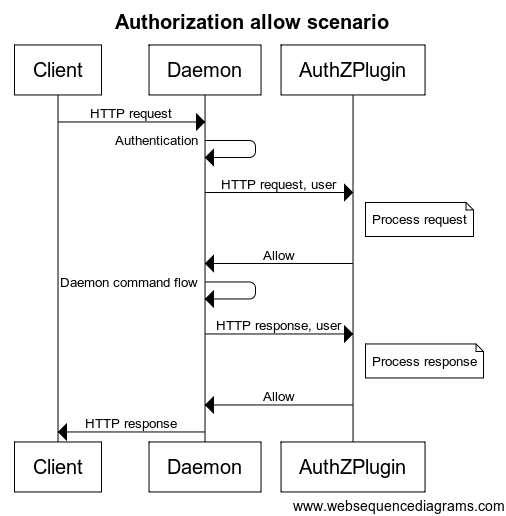
\includegraphics[width=0.9\textwidth]{./images/sec_authzAllow.png}
        %\caption{Ablaufdiagramm einer Befehlsausführung mit \emph{AuthZ} im Fall einer erfolgreichen Authorisierung \cite{githubAuthZExtended}.}
        %\label{fig:sec_authzAllow}
    %\end{figure}

    %\begin{figure}[h]
        %\centering
        %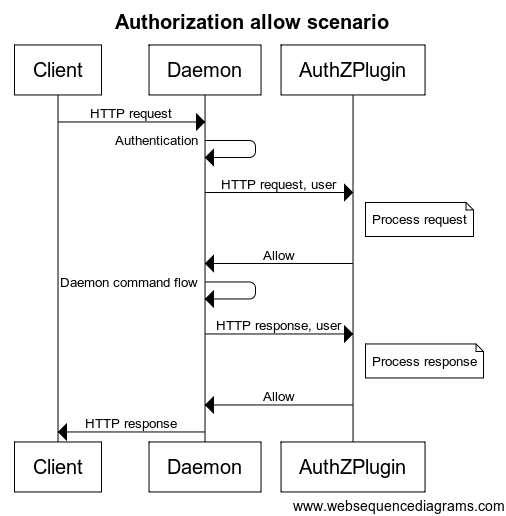
\includegraphics[width=0.9\textwidth]{./images/sec_authzAllow.png}
        %\caption{Ablaufdiagramm einer Befehlsausführung mit \emph{AuthZ} im Fall einer fehlgeschlagenen Authorisierung \cite{githubAuthZExtended}.}
        %\label{fig:sec_authzDeny}
    %\end{figure}

    \begin{figure}
      \centering
      \begin{subfigure}{.5\textwidth}
        \centering
        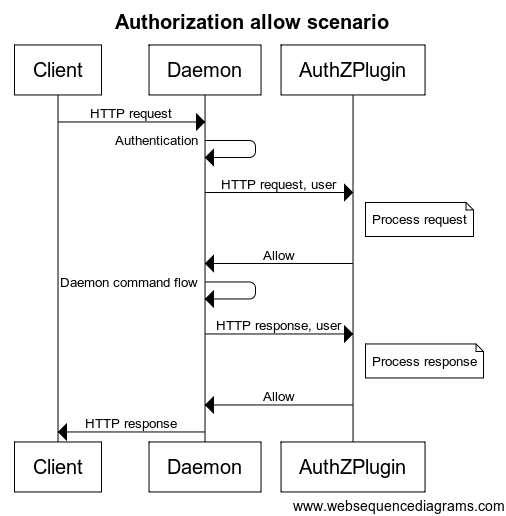
\includegraphics[width=1.0\linewidth]{./images/sec_authzAllow.png}
        \caption{Erfolgreiche Authorisierung}
        \label{fig:sec_authzAllow}
      \end{subfigure}%
      \begin{subfigure}{.5\textwidth}
        \centering
        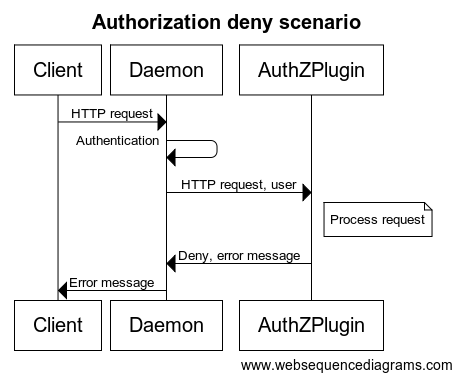
\includegraphics[width=1.0\linewidth]{./images/sec_authzDeny.png}
        \caption{Fehlgeschlagene Authorisierung}
        \label{fig:sec_authzDeny}
      \end{subfigure}
      \caption{Ablaufdiagramm einer Befehlsausführung mit dem Authorisierungs-Plugins \emph{AuthZ} von Docker \cite{githubAuthZExtended}.}
      \label{fig:sec_authz}
    \end{figure}
    % (TODO): Evtl. untereinander machen da zu wenig Platz. Oder Grafik neu machen mit weniger/groesserem Text
    % Laut Patrick: Groesse OK!


    Die Struktur von Anfragen und Antworten, die über das HTTP-Protokoll ausgetauscht werden, sind in \cite{githubAuthZExtended} spezifiziert.

    Mehrere Sicherheitsmodule können konsekutiv ausgeführt werden, sodass jeder clientseitigen Interaktion mit dem Daemon, die Ausführung mehrerer \emph{AuthZ}-Implementierungen folgt.

    Mit folgender Syntax können Authorisierungs-Plugins für den Daemon aktiviert werden \cite{githubAuthZExtended}:

    \begin{lstlisting}
      docker daemon --authorization-plugin=PLUGIN1 \
                   [--authorization-plugin=PLUGIN2] [...]
    \end{lstlisting}

    Da es sich bei diesen sicherheitsrelevanten Plugins um ein sehr neues Feature von Docker handelt, war die offizielle Dokumentation zum Zeitpunkt der Erstellung dieser Arbeit nicht vollständig. Insbesondere die fehlende Spezifikation des Formats eines \emph{AuthZ}-Regelwerks im Docker-Repository lässt vermuten, dass eine vollständige Einführung von \emph{AuthZ} erst im Rahmen zukünftiger Docker-Veröffentlichungen stattfindet.

  \section{Open-Source-Charakter und Sicherheitspolitik von Docker}
  \label{opensource}
    Docker ist wie Linux ein Open-Source-Projekt, das nicht nur von Docker-Mitarbeitern entwickelt wird, sondern die Unterstützung vieler freiwilliger Entwickler und Sicherheitsexperten findet. Der Open-Source-Charakter von Docker und Software allgemein kann jedoch aus Sicherheitssicht kontrovers diskutiert werden:

    \paragraph{Vorteile:}
    \begin{itemize}
      \item Durch die Vielzahl an Involvierten können Sicherheitslücken schneller entdeckt und behoben werden. Über 1300 Individuen haben sich bislang für die Weiterentwicklung der Codebasis und der Aufdeckung von Fehlern und Sicherheitsrisiken an Docker beteiligt.
      %Die Codequalität profitiert auch von Experten anderer Unternehmen und Organisationen, im Docker-Projekt z.\,B. von \emph{Red Hat}-Mitarbeitern.
      \item Eigene Sicherheitspraktiken können von Anwendern durch die Kenntnis über den Quellcode hinzugefügt werden.
      \item Nach dem \emph{Kerkhoffs'schen Prinzip} ist einer Anwendung von \emph{Security Through Obscurity} generell abzuraten. Ein offenes Design von Serversystemen ist von NIST als allgemeines Sicherheitsprinzip vorgeschlagen \cite[S.15]{nist}.
    \end{itemize}

    \paragraph{Nachteile:}
    \begin{itemize}
      \item Sicherheitslücken sind von Angreifern prinzipiell schneller zu finden, wenn diese im Besitz des Quellcodes sind.
      \item Durch die lose Zusammenarbeit vieler Experten ist nicht gewährleistet, dass bestimmte Implementierungen nach dem Mehraugenprinzip kontrolliert werden. Die böswillige Absicht nur eines Entwicklers kann in einer Open-Source-Kultur weiterhin starke Beeinträchtigungen der Sicherheit mit sich bringen.
    \end{itemize}

    Die Vor- und Nachteile zeigen auf, dass es keinen eindeutigen Gewinner nach Maßstäben der Sicherheit gibt. Sowohl Open-Source- als auch proprietäre Softwarelösungen können erfolgreich sein, wie die Vergangenheit bekannter Betriebssysteme und Anwendungen zeigt. Für \emph{Docker} hat sich der Open-Source-Ansatz bislang bewährt.

    Um die Zusammenarbeit im Docker-Projekt zu organisieren, wurden Regeln und Konventionen formuliert, die auch die Sicherheit betreffen \cite{githubDockerContribution}. Zusammen mit den Sicherheitsrichtlinien aus der offiziellen Docker-Homepage, ergeben sich folgende weitere, sicherheitsrelevante Eigenschaften von Docker.

    \begin{itemize}
      \item Prinzip von \emph{Responsible Disclosure} wird als Hauptbestandteil der Sicherheitspolitik von Docker umgesetzt. Konform dazu können entdeckte Schwachstellen jederzeit an eine zentrale E-Mail-Adresse kommuniziert werden \cite{dockerSecurityPortal}.
      \item Wartung einer zentralen \acrshort{CVE}-Datenbank, die bekannte Sicherheitsrisiken von Docker enthält. Die darin veröffentlichten Informationen erfüllen das Prinzip \emph{Responsible Disclosure} \cite{dockerCVEList}.
      \item Externe Sicherheitsfirmen werden vierteljährlich beauftragt, Sicherheitsaudits und Penetrationstests zur Kontrolle der Codebasis und Infrastruktur durchzuführen \cite[S.5]{dockerSecIntro}.
    \end{itemize}

  \section{Best-Practices für die Sicherheit}
    In den folgenden Abschnitten sind verschiedene Best-Practices im Umgang mit Docker aufgezählt.

    Während insgesamt weitaus mehr Best-Pracices existieren, sind im Folgenden nur jene ausgewählt, die Bezug zu den meisten Anwendungsfällen haben.

    \subsection{Skripte}
      Es existieren Skripte, die Docker"=Hostsysteme nach eingehaltenen und nicht erfüllten Best-Practices überprüfen.

      Der bekannteste Vertreter ist \emph{Docker Bench} \cite{githubDockerBench}, welcher in das Docker-Projekt integriert ist und nach Aussagen der Entwickler auf Befunden des Sicherheitsberichts des unabhängigen \emph{Center for Internet Security} beruht \cite{dockerBenchmarkCIS}. Dieser Bericht ist im Mai 2015 entstanden und enthält sicherheitsrelevante Befunde zu Docker in der Version 1.6. Aktuellere Berichte zu moderneren Docker-Versionen existieren nicht.

      Die darin enthaltenen Kontrollen sind in einem eigenen Image als Shellskripte definiert. Zur Ausführung der Tests muss dieses Image als Container gestartet werden. Im Rahmen dieser Tests werden direkt über Shellbefehle abrufbare Parameter untersucht. Darunter sind z.\,B.:

      \begin{itemize}
        \item Rechte, Besitzer- und Gruppenzugehörigkeiten von Dateien und Verzeichnissen
        \item Docker- und Kernelversion
        \item Log- und Netzwerkeinstellungen
        \item TLS-Unterstützung
        \item Existenz von (nicht-)priveligierten Containern
        \item Verwendung von Capabilities, \emph{AppArmor}- und \emph{SELinux}-Profilen
      \end{itemize}

      Die konkreten Tests sind unter \cite{githubDockerBenchTests} in ihrer aktuellsten Version im Detail veröffentlicht.

    \subsection{Datencontainer}
      Die von Werkzeugen wie \emph{Docker Bench} ausführbare Tests beschränken sich auf explizit abrufbare Parameter des Hosts und von Docker. In Serverinfrastrukturen existieren jedoch auch Sicherheitskriterien, deren Kontrolle nicht über Abfragen von Einstellungen des Hostsystems oder von Docker abzudecken ist. Insbesondere Merkmale der Infrastuktur wirken sich auf die Verfügbarkeit von Diensten sowie der Wartbarkeit einer Infrastruktur aus.

      Aus diesem Grund wird von \emph{Docker} empfohlen, eigene Datencontainer zu betreiben, über die Anwendungen anderer Container ihren Zustand auf Datenebene persistieren können. Anwendungen können in diesem Szenario über mehrere Container hinweg auf den Datencontainer zugreifen, sofern letzterer Methoden implementiert, um Race-Conditions zu verarbeiten. Standardmäßig gehen Änderungen, die während dem Betrieb von Containern auftreten, verloren, sobald der Container gestoppt wird. Diese Eigenschaft beruht auf der obersten Schicht eines Containers, die bei Containerstart einem Image hinzugefügt wird. Dieser Layer ist unabhängig von dem zugrundeliegendem Image und existiert nur temporär zur Laufzeit des Containers.

      Dieser Eigenschaft unterliegen auch Datencontainer. Deshalb empfiehlt es sich, die Verzeichnisse von Datencontainern aus dem Hostsystem über Mounts einzubinden. Welche Verzeichnisse des Hostsystems über Datencontainer für Anwendungscontainer verfügbar sind, kann in Datencontainern zentral eingestellt werden \cite{dockerManageDataContainers}.
      % TODO: Referenz zu Grundlagenkapitel "Einführung in Docker"

      % mounts von normalen servicecontainern werden vermieden.
      % "Zustand/State" ist getrennt

    \subsection{Verwaltung von Credentials}
      Informationen zu Benutzernamen und Passwörtern sollten nicht statisch als Zeichenketten in ein Image integriert sein. Vielmehr sollen Credentials generell als Umgebungsvariablen mit der \texttt{ENV}-Direktive der Dockerfiles in Images verfügbar gemacht werden.

      Beispielsweise setzen die Entwickler von der Datenbank \emph{Postgres} diese Praxis in ihrem \emph{Postgres}-Image um, indem sie die Umgebungsvariablen \texttt{POSTGRES\_USER} und \texttt{POSTGRES\_PASSWORD} definieren, die beim Startvorgang des Containers abgefragt werden \cite{dockerHubPostgres}\cite{githubPostgresCredentialCheck}.

  \section{Tools}
    Im Docker-Ökosystem existieren zahlreiche Tools, die entweder den Funktionsumfang von Docker erweitern oder zusätzliche Möglichkeiten bieten, Docker-Container zu verwalten. Neben Veröffentlichungen von \emph{Docker}, z.\,B. mit \emph{Docker Swarm}, \emph{Docker Compose} und \emph{Docker Datacenter}, können auch einige Entwicklungen von Drittanbietern verwendet werden. Diese umfassen beispielsweise \emph{Kubernetes} \cite{kubernetes}, \emph{Shipyard} \cite{shipyard} und \emph{docker-slim} \cite{githubDockerSlim}. Die genannten Tools decken teilweise gleiche Features ab oder bauen im Fall von \emph{Docker Swarm} und \emph{Shipyard} aufeinander auf.

    Viele erweiternde Features werden von Docker auch mittels der Schnittstelle Docker-Plugins unterstützt. Die sicherheitsrelevante Erweiterung \emph{AuthZ} wurde bereits in Abschnitt \ref{plugins} vorgestellt.

    Im Folgenden werden ausgewählte Werkzeuge kurz vorgestellt. Außerdem wird erörtert, inwiefern sie zur Sicherheit von Docker beitragen und welche von Docker unabhängigen Sicherheitsfunktionen sie anbieten.
    % Der CEO von \emph{Docker}, Solomon Hykes, sieht den Fokus des Unternehmens zukünftig in den Werkzeugen, die Images und Container begleiten. Aus diesem Grund ist \emph{Docker} sehr bemüht, hauseigene Erweiterungen wie das jüngst erschienene \emph{Docker Datacenter} zu etablieren.
    % Oder Aufteilung in DevOops Tools (Puppet, Ansible, Vagrant) und Orchestrierungstools (Mesos, Shipyard, Kubernetes)
    % Diese Tools bieten eine weitere Abstraktionsschicht für den Betrieb von Docker-Containern.

    % TODO: Twistlock nicht mehr explizit aufgefuhert, da in Docker-Release seit V.1.10 integriert.
    % s. www.twistlock.com

    % Viele Tools/Plugins parallel zu Docker entstanden, um in den Bereichen Volume,Networking,Security nachzulegen.
    % s. https://github.com/docker/docker/blob/master/docs/extend/plugins.md
    % Vieles in Docker-main integriert oder pluggable gemacht mit plugin framework.

    \subsection{Kubernetes}
      %\emph{orchestration, management fokus, sicherheitsrelevant?}
      % neueres Cluster-Management Tool von Google
      % Hat Relevanz fuer Herr Fahner/Daimler
      Als ausgewählter Vertreter der Verwaltungs- und Orchestrierungswerkzeuge wird in diesem Abschnitt das von \emph{Google} entwickelte Open-Source-Werkzeug \emph{Kubernetes} und dessen Sicherheitsverständnis vorgestellt.

      Der Fokus von \emph{Kubernetes} liegt auf der Verwaltung und Orchestrierung von Containern, die über mehrere Hosts verteilt sind. Damit eignet sich das Tool v.\,a. in Cloud"=Infrastrukturen, welche sich i.d.R. aus mehreren, über das Netzwerk miteinander verbundenen Hostsystemen zusammensetzen. Es führt neue Konzepte ein, um eine Vielzahl von Containern auf physischen und virtuellen Systemen zu verwalten.

      %Neben einigen Startups, haben sich \emph{Google}, \emph{Microsoft}, \emph{VMware}, \emph{IBM} und \emph{Red Hat} als \emph{Kubernetes}-Unterstützer geäußert.

      Aus der Sicht von \emph{Kubernetes} stellen z.\,B. Docker-Container die kleinste zu verwaltende Einheit dar. Welche Anwendung in einem Container läuft und welche Sicherheitsmechanismen aus Kapitel \ref{secLinux} der Container nutzt, um das jeweilige Hostsystem zu schützen, ist für den Betrieb von \emph{Kubernetes} zunächst unerheblich.

      \emph{Kubernetes} erfüllt hauptsächlich administrative Anforderungen an die Sicherheit, die auch hier wieder auf Basis des \emph{Principle of Least Privilege} umgesetzt werden. Damit ist die Implementierung einer rollenbasierten Nutzerkontrolle (\acrshort{RBAC}) gemeint, die Nutzer über alle von Kubernetes kontrollierten Container hinweg, authorisiert und authentifiziert \cite{githubKubernetesSecurity}. Im Vergleich dazu ermöglicht die Verwendung des Authentifizierungs-Framework \emph{AuthZ} aus Kapitel \ref{plugins} nur die Authentifizierung von Nutzern auf einem Hostsystem.

      % TODO: Vieles was Kubernetes macht, passiert auf Netzwerkebene. Und das nicht in dieser Arbeit.

      % Ein Hauptfeature von Containern ist deren flexibler Einsatz in Anwendungsclustern, die eine Multi-Tier-Anwendung / Multi-Tenant-Architektur abbilden.
      % Im Juni 2014 hat Google das Open-Source Tool \emph{Kubernetes} angekündigt, das Cluster mit Docker-Containern verwalten soll. Laut Google ist Kubernetes die Entkopplung von Anwendungscontainern von Details des Hosts.
      % Soll in Datencentern die Arbeit mit Containern vereinfachen.
      % (Bringt angeblich tolles Networking-Feature mit.)

    \subsection{docker-slim}
      \emph{docker-slim} ist ein Werkzeug, das u.\,a. automatisch Sicherheitsprofile erstellt. Es untersucht dabei Anwendungen, die in einem Container laufen und zeichnet Zugriffe dieser auf, z.\,B. die verwendeten \emph{System Calls}. Aus diesen Aufzeichnungen und einer Analyse der statischen Daten eines Images werden Profile für \emph{Seccomp} und \emph{AppArmor} erstellt, die anschließend verwendet werden können. Die Generierung eines \emph{AppArmor}-Profils ist aktuell in der Entwicklungsphase \cite{githubDockerSlim}.

    \subsection{Bane}
      Auch das von Docker-Mitarbeiterin Jessie Frazelle entwickelte Werkzeug \emph{Bane} hat zum Ziel, \emph{AppArmor}-Profile automatisch zu generieren. Im Gegensatz zu \emph{docker-slim} analysiert es nicht Images und Container, sondern übersetzt Anweisungen einer gut lesbaren Konfigurationsdatei in ein \emph{AppArmor}-Profil. Der Vorteil der Konfigurationsdatei gegenüber einer Datei, die ein \emph{AppArmor}-Profil enthält, ist, dass sich ausdruckstärkere, kategorisierbare Anweisungen formulieren lassen, sodass zum Erstellen der Datei keine speziellen \emph{AppArmor}-Kenntnisse erforderlich sind \cite{githubBane}.

      Ein beispielhafter Ausschnitt einer Konfigurationsdatei im \acrshort{TOML}-Format könnte folgendermaßen aussehen \cite{githubBaneTOML}:

      \begin{lstlisting}
        ...
        [Filesystem]
        WritablePaths = [
        	"/var/run/nginx.pid"
        ]
        AllowExec = [
        	"/usr/sbin/nginx"
        ]
        DenyExec = [
        	"/bin/sh",
        	"/usr/bin/top"
        ]
        ...
      \end{lstlisting}

      Bei der Übersetzung in ein valides \emph{AppArmor}-Profil, entstehen daraus folgende Zeilen \cite{githubBaneAppArmorSample}:

      \begin{lstlisting}
        ...
        /var/run/nginx.pid w,
        /usr/sbin/nginx ix,
        deny /bin/sh mrwklx,
        deny /usr/bin/top mrwklx,
        ...
      \end{lstlisting}

      Wie bei einem Vergleich der beiden Fragmente zu sehen ist, ist die Konfigurationsdatei strukturierter und durch Verwendung von aussagekräftigen Bezeichnern wie \texttt{Filesystem}, \texttt{WritablePaths}, \texttt{AllowExec} und \texttt{DenyExec} übersichtlicher als das daraus generierte \emph{AppArmor}-Profil.

      Nach Aussage von Jessie Frazelle in
      \cite{githubBane}, \cite{githubGeneralSecProfiles}
      und \cite{docker110Security} stellt \emph{Bane} den Grundbaustein eines zukünftigen universalen, nativen Sicherheitmoduls mit Profilen für Capabilities, \emph{AppArmor} und \emph{Seccomp} dar. Dieses wird voraussichtlich in eine zukünftige Docker-Version einfließen.

\end{document}
